\documentclass[twoside]{book}

% Packages required by doxygen
\usepackage{fixltx2e}
\usepackage{calc}
\usepackage{doxygen}
\usepackage[export]{adjustbox} % also loads graphicx
\usepackage{graphicx}
\usepackage[utf8]{inputenc}
\usepackage{makeidx}
\usepackage{multicol}
\usepackage{multirow}
\PassOptionsToPackage{warn}{textcomp}
\usepackage{textcomp}
\usepackage[nointegrals]{wasysym}
\usepackage[table]{xcolor}

% Font selection
\usepackage[T1]{fontenc}
\usepackage[scaled=.90]{helvet}
\usepackage{courier}
\usepackage{amssymb}
\usepackage{sectsty}
\renewcommand{\familydefault}{\sfdefault}
\allsectionsfont{%
  \fontseries{bc}\selectfont%
  \color{darkgray}%
}
\renewcommand{\DoxyLabelFont}{%
  \fontseries{bc}\selectfont%
  \color{darkgray}%
}
\newcommand{\+}{\discretionary{\mbox{\scriptsize$\hookleftarrow$}}{}{}}

% Page & text layout
\usepackage{geometry}
\geometry{%
  a4paper,%
  top=2.5cm,%
  bottom=2.5cm,%
  left=2.5cm,%
  right=2.5cm%
}
\tolerance=750
\hfuzz=15pt
\hbadness=750
\setlength{\emergencystretch}{15pt}
\setlength{\parindent}{0cm}
\setlength{\parskip}{3ex plus 2ex minus 2ex}
\makeatletter
\renewcommand{\paragraph}{%
  \@startsection{paragraph}{4}{0ex}{-1.0ex}{1.0ex}{%
    \normalfont\normalsize\bfseries\SS@parafont%
  }%
}
\renewcommand{\subparagraph}{%
  \@startsection{subparagraph}{5}{0ex}{-1.0ex}{1.0ex}{%
    \normalfont\normalsize\bfseries\SS@subparafont%
  }%
}
\makeatother

% Headers & footers
\usepackage{fancyhdr}
\pagestyle{fancyplain}
\fancyhead[LE]{\fancyplain{}{\bfseries\thepage}}
\fancyhead[CE]{\fancyplain{}{}}
\fancyhead[RE]{\fancyplain{}{\bfseries\leftmark}}
\fancyhead[LO]{\fancyplain{}{\bfseries\rightmark}}
\fancyhead[CO]{\fancyplain{}{}}
\fancyhead[RO]{\fancyplain{}{\bfseries\thepage}}
\fancyfoot[LE]{\fancyplain{}{}}
\fancyfoot[CE]{\fancyplain{}{}}
\fancyfoot[RE]{\fancyplain{}{\bfseries\scriptsize Generated by Doxygen }}
\fancyfoot[LO]{\fancyplain{}{\bfseries\scriptsize Generated by Doxygen }}
\fancyfoot[CO]{\fancyplain{}{}}
\fancyfoot[RO]{\fancyplain{}{}}
\renewcommand{\footrulewidth}{0.4pt}
\renewcommand{\chaptermark}[1]{%
  \markboth{#1}{}%
}
\renewcommand{\sectionmark}[1]{%
  \markright{\thesection\ #1}%
}

% Indices & bibliography
\usepackage{natbib}
\usepackage[titles]{tocloft}
\setcounter{tocdepth}{3}
\setcounter{secnumdepth}{5}
\makeindex

% Hyperlinks (required, but should be loaded last)
\usepackage{ifpdf}
\ifpdf
  \usepackage[pdftex,pagebackref=true]{hyperref}
\else
  \usepackage[ps2pdf,pagebackref=true]{hyperref}
\fi
\hypersetup{%
  colorlinks=true,%
  linkcolor=blue,%
  citecolor=blue,%
  unicode%
}

% Custom commands
\newcommand{\clearemptydoublepage}{%
  \newpage{\pagestyle{empty}\cleardoublepage}%
}

\usepackage{caption}
\captionsetup{labelsep=space,justification=centering,font={bf},singlelinecheck=off,skip=4pt,position=top}

%===== C O N T E N T S =====

\begin{document}

% Titlepage & ToC
\hypersetup{pageanchor=false,
             bookmarksnumbered=true,
             pdfencoding=unicode
            }
\pagenumbering{roman}
\begin{titlepage}
\vspace*{7cm}
\begin{center}%
{\Large Tratamento de Classes Abstratas \\[1ex]\large 0.\+0.\+1 }\\
\vspace*{1cm}
{\large Generated by Doxygen 1.8.11}\\
\end{center}
\end{titlepage}
\clearemptydoublepage
\tableofcontents
\clearemptydoublepage
\pagenumbering{arabic}
\hypersetup{pageanchor=true}

%--- Begin generated contents ---
\chapter{Tratamento de Classes Abstratas}
\label{md_README}
\hypertarget{md_README}{}
{\itshape 2ª parte do projeto da segunda unidade da disciplina de Programação Avançada (dca1202) referente a utilização de Classes Abstratas para manipulação de figuras geométricas.}


\begin{DoxyItemize}
\item O projeto segue as especificações contidas \href{http://agostinhobritojr.github.io/cursos/progav/projetoscpp.html#_projeto_2_tratamento_de_classes_abstratas}{\tt nesta página}
\end{DoxyItemize}

\subsection*{Membros do projeto}


\begin{DoxyItemize}
\item Francisco Mateus de Oliveira Abrantes
\item Isaac Gomes de Oliveira 
\end{DoxyItemize}
\chapter{Hierarchical Index}
\section{Class Hierarchy}
This inheritance list is sorted roughly, but not completely, alphabetically\+:\begin{DoxyCompactList}
\item \contentsline{section}{Poligono}{\pageref{class_poligono}}{}
\begin{DoxyCompactList}
\item \contentsline{section}{Retangulo}{\pageref{class_retangulo}}{}
\end{DoxyCompactList}
\item \contentsline{section}{Ponto}{\pageref{class_ponto}}{}
\end{DoxyCompactList}

\chapter{Class Index}
\section{Class List}
Here are the classes, structs, unions and interfaces with brief descriptions\+:\begin{DoxyCompactList}
\item\contentsline{section}{\hyperlink{class_poligono}{Poligono} \\*A classe \hyperlink{class_poligono}{Poligono} representa polígonos convexos de até 100 vértices }{\pageref{class_poligono}}{}
\item\contentsline{section}{\hyperlink{class_ponto}{Ponto} \\*A classe \hyperlink{class_ponto}{Ponto} representa pontos no espaço bidimensional }{\pageref{class_ponto}}{}
\item\contentsline{section}{\hyperlink{class_retangulo}{Retangulo} }{\pageref{class_retangulo}}{}
\end{DoxyCompactList}

\chapter{File Index}
\section{File List}
Here is a list of all files with brief descriptions\+:\begin{DoxyCompactList}
\item\contentsline{section}{Qt\+Tcp\+Server/\hyperlink{datastorage_8cpp}{datastorage.\+cpp} }{\pageref{datastorage_8cpp}}{}
\item\contentsline{section}{Qt\+Tcp\+Server/\hyperlink{datastorage_8h}{datastorage.\+h} }{\pageref{datastorage_8h}}{}
\item\contentsline{section}{Qt\+Tcp\+Server/\hyperlink{main_8cpp}{main.\+cpp} }{\pageref{main_8cpp}}{}
\item\contentsline{section}{Qt\+Tcp\+Server/\hyperlink{mainwindow_8cpp}{mainwindow.\+cpp} }{\pageref{mainwindow_8cpp}}{}
\item\contentsline{section}{Qt\+Tcp\+Server/\hyperlink{mainwindow_8h}{mainwindow.\+h} }{\pageref{mainwindow_8h}}{}
\item\contentsline{section}{Qt\+Tcp\+Server/\hyperlink{moc__mainwindow_8cpp}{moc\+\_\+mainwindow.\+cpp} }{\pageref{moc__mainwindow_8cpp}}{}
\item\contentsline{section}{Qt\+Tcp\+Server/\hyperlink{moc__myserver_8cpp}{moc\+\_\+myserver.\+cpp} }{\pageref{moc__myserver_8cpp}}{}
\item\contentsline{section}{Qt\+Tcp\+Server/\hyperlink{moc__mythread_8cpp}{moc\+\_\+mythread.\+cpp} }{\pageref{moc__mythread_8cpp}}{}
\item\contentsline{section}{Qt\+Tcp\+Server/\hyperlink{myserver_8cpp}{myserver.\+cpp} }{\pageref{myserver_8cpp}}{}
\item\contentsline{section}{Qt\+Tcp\+Server/\hyperlink{myserver_8h}{myserver.\+h} }{\pageref{myserver_8h}}{}
\item\contentsline{section}{Qt\+Tcp\+Server/\hyperlink{mythread_8cpp}{mythread.\+cpp} }{\pageref{mythread_8cpp}}{}
\item\contentsline{section}{Qt\+Tcp\+Server/\hyperlink{mythread_8h}{mythread.\+h} }{\pageref{mythread_8h}}{}
\item\contentsline{section}{Qt\+Tcp\+Server/\hyperlink{ui__mainwindow_8h}{ui\+\_\+mainwindow.\+h} }{\pageref{ui__mainwindow_8h}}{}
\end{DoxyCompactList}

\chapter{Class Documentation}
\hypertarget{class_circulo}{}\section{Circulo Class Reference}
\label{class_circulo}\index{Circulo@{Circulo}}


A classe \hyperlink{class_circulo}{Circulo} cria um objeto do tipo \hyperlink{class_circulo}{Circulo} que pode ser desenhada numa \hyperlink{class_screen}{Screen}.  




{\ttfamily \#include $<$circulo.\+h$>$}



Inheritance diagram for Circulo\+:
\nopagebreak
\begin{figure}[H]
\begin{center}
\leavevmode
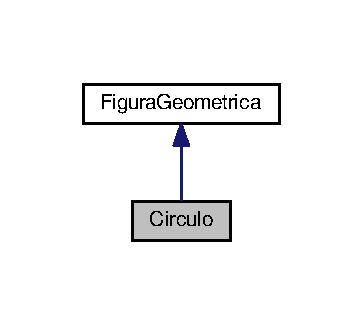
\includegraphics[width=174pt]{class_circulo__inherit__graph}
\end{center}
\end{figure}


Collaboration diagram for Circulo\+:
\nopagebreak
\begin{figure}[H]
\begin{center}
\leavevmode
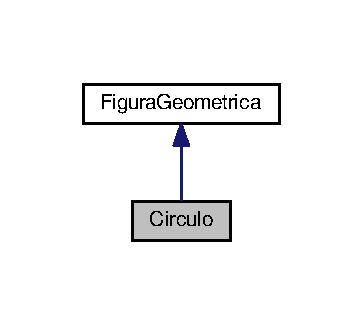
\includegraphics[width=174pt]{class_circulo__coll__graph}
\end{center}
\end{figure}
\subsection*{Public Member Functions}
\begin{DoxyCompactItemize}
\item 
\hyperlink{class_circulo_ae86b351de917e3fede1d43e8495b1979}{Circulo} (int \+\_\+x0, int \+\_\+y0, int \+\_\+raio, bool \+\_\+fillmode, char \+\_\+brush=\textquotesingle{}$\ast$\textquotesingle{})
\begin{DoxyCompactList}\small\item\em \hyperlink{class_circulo}{Circulo} é o construtor da classe \hyperlink{class_circulo}{Circulo}. \end{DoxyCompactList}\item 
void \hyperlink{class_circulo_a593787d6e0618c2eded23e8839e7bea6}{draw} (\hyperlink{class_screen}{Screen} \&t)
\begin{DoxyCompactList}\small\item\em draw desenha um \hyperlink{class_circulo}{Circulo} numa tela \end{DoxyCompactList}\end{DoxyCompactItemize}


\subsection{Detailed Description}
A classe \hyperlink{class_circulo}{Circulo} cria um objeto do tipo \hyperlink{class_circulo}{Circulo} que pode ser desenhada numa \hyperlink{class_screen}{Screen}. 

Esta classe extende a classe \hyperlink{class_figura_geometrica}{Figura\+Geometrica} 

\subsection{Constructor \& Destructor Documentation}
\index{Circulo@{Circulo}!Circulo@{Circulo}}
\index{Circulo@{Circulo}!Circulo@{Circulo}}
\subsubsection[{\texorpdfstring{Circulo(int \+\_\+x0, int \+\_\+y0, int \+\_\+raio, bool \+\_\+fillmode, char \+\_\+brush=\textquotesingle{}$\ast$\textquotesingle{})}{Circulo(int _x0, int _y0, int _raio, bool _fillmode, char _brush='*')}}]{\setlength{\rightskip}{0pt plus 5cm}Circulo\+::\+Circulo (
\begin{DoxyParamCaption}
\item[{int}]{\+\_\+x0, }
\item[{int}]{\+\_\+y0, }
\item[{int}]{\+\_\+raio, }
\item[{bool}]{\+\_\+fillmode, }
\item[{char}]{\+\_\+brush = {\ttfamily \textquotesingle{}$\ast$\textquotesingle{}}}
\end{DoxyParamCaption}
)}\hypertarget{class_circulo_ae86b351de917e3fede1d43e8495b1979}{}\label{class_circulo_ae86b351de917e3fede1d43e8495b1979}


\hyperlink{class_circulo}{Circulo} é o construtor da classe \hyperlink{class_circulo}{Circulo}. 


\begin{DoxyParams}{Parameters}
{\em \+\_\+x0} & é a coordenada x do centro do \hyperlink{class_circulo}{Circulo} \\
\hline
{\em \+\_\+y0} & é a coordenada y do centro do \hyperlink{class_circulo}{Circulo} \\
\hline
{\em \+\_\+raio} & é o raio do \hyperlink{class_circulo}{Circulo} \\
\hline
{\em \+\_\+fillmode} & indica se o \hyperlink{class_circulo}{Circulo} deve ser preenchido ou não \\
\hline
{\em \+\_\+brush} & indica o caraceter a ser utilizado para desenhar o \hyperlink{class_circulo}{Circulo} \\
\hline
\end{DoxyParams}


\subsection{Member Function Documentation}
\index{Circulo@{Circulo}!draw@{draw}}
\index{draw@{draw}!Circulo@{Circulo}}
\subsubsection[{\texorpdfstring{draw(\+Screen \&t)}{draw(Screen &t)}}]{\setlength{\rightskip}{0pt plus 5cm}void Circulo\+::draw (
\begin{DoxyParamCaption}
\item[{{\bf Screen} \&}]{t}
\end{DoxyParamCaption}
)\hspace{0.3cm}{\ttfamily [virtual]}}\hypertarget{class_circulo_a593787d6e0618c2eded23e8839e7bea6}{}\label{class_circulo_a593787d6e0618c2eded23e8839e7bea6}


draw desenha um \hyperlink{class_circulo}{Circulo} numa tela 


\begin{DoxyParams}{Parameters}
{\em t} & é a tela na qual se deseja desenhar \\
\hline
\end{DoxyParams}


Implements \hyperlink{class_figura_geometrica_a8ee8dedc060b6059a805ea091aef2c41}{Figura\+Geometrica}.



The documentation for this class was generated from the following files\+:\begin{DoxyCompactItemize}
\item 
\hyperlink{circulo_8h}{circulo.\+h}\item 
\hyperlink{circulo_8cpp}{circulo.\+cpp}\end{DoxyCompactItemize}

\hypertarget{class_figura_geometrica}{}\section{Figura\+Geometrica Class Reference}
\label{class_figura_geometrica}\index{Figura\+Geometrica@{Figura\+Geometrica}}


A classe \hyperlink{class_figura_geometrica}{Figura\+Geometrica} é uma classe abstrata que desenha Figuras Geometricas.  




{\ttfamily \#include $<$figurageometrica.\+h$>$}



Inheritance diagram for Figura\+Geometrica\+:
\nopagebreak
\begin{figure}[H]
\begin{center}
\leavevmode
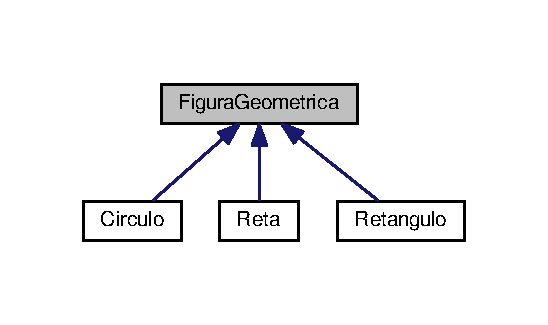
\includegraphics[width=263pt]{class_figura_geometrica__inherit__graph}
\end{center}
\end{figure}
\subsection*{Public Member Functions}
\begin{DoxyCompactItemize}
\item 
\hyperlink{class_figura_geometrica_a81d7c7efaea511e60a15f5a363138dd9}{Figura\+Geometrica} ()
\begin{DoxyCompactList}\small\item\em \hyperlink{class_figura_geometrica}{Figura\+Geometrica} é o construtor da classe \hyperlink{class_figura_geometrica}{Figura\+Geometrica}. \end{DoxyCompactList}\item 
virtual void \hyperlink{class_figura_geometrica_a8ee8dedc060b6059a805ea091aef2c41}{draw} (\hyperlink{class_screen}{Screen} \&t)=0
\begin{DoxyCompactList}\small\item\em draw é o método da classe Abstrata que ira desenhar objetos de outras classes que implementam esse método \end{DoxyCompactList}\end{DoxyCompactItemize}


\subsection{Detailed Description}
A classe \hyperlink{class_figura_geometrica}{Figura\+Geometrica} é uma classe abstrata que desenha Figuras Geometricas. 

\subsection{Constructor \& Destructor Documentation}
\index{Figura\+Geometrica@{Figura\+Geometrica}!Figura\+Geometrica@{Figura\+Geometrica}}
\index{Figura\+Geometrica@{Figura\+Geometrica}!Figura\+Geometrica@{Figura\+Geometrica}}
\subsubsection[{\texorpdfstring{Figura\+Geometrica()}{FiguraGeometrica()}}]{\setlength{\rightskip}{0pt plus 5cm}Figura\+Geometrica\+::\+Figura\+Geometrica (
\begin{DoxyParamCaption}
{}
\end{DoxyParamCaption}
)}\hypertarget{class_figura_geometrica_a81d7c7efaea511e60a15f5a363138dd9}{}\label{class_figura_geometrica_a81d7c7efaea511e60a15f5a363138dd9}


\hyperlink{class_figura_geometrica}{Figura\+Geometrica} é o construtor da classe \hyperlink{class_figura_geometrica}{Figura\+Geometrica}. 



\subsection{Member Function Documentation}
\index{Figura\+Geometrica@{Figura\+Geometrica}!draw@{draw}}
\index{draw@{draw}!Figura\+Geometrica@{Figura\+Geometrica}}
\subsubsection[{\texorpdfstring{draw(\+Screen \&t)=0}{draw(Screen &t)=0}}]{\setlength{\rightskip}{0pt plus 5cm}virtual void Figura\+Geometrica\+::draw (
\begin{DoxyParamCaption}
\item[{{\bf Screen} \&}]{t}
\end{DoxyParamCaption}
)\hspace{0.3cm}{\ttfamily [pure virtual]}}\hypertarget{class_figura_geometrica_a8ee8dedc060b6059a805ea091aef2c41}{}\label{class_figura_geometrica_a8ee8dedc060b6059a805ea091aef2c41}


draw é o método da classe Abstrata que ira desenhar objetos de outras classes que implementam esse método 


\begin{DoxyParams}{Parameters}
{\em t} & é a tela na qual se deseja desenhar \\
\hline
\end{DoxyParams}


Implemented in \hyperlink{class_circulo_a593787d6e0618c2eded23e8839e7bea6}{Circulo}, \hyperlink{class_retangulo_ac088dd6d3f4f3d3f80363a868c2e74f1}{Retangulo}, and \hyperlink{class_reta_ac2e9805183cd474b62bffd8b032cd780}{Reta}.



The documentation for this class was generated from the following files\+:\begin{DoxyCompactItemize}
\item 
\hyperlink{figurageometrica_8h}{figurageometrica.\+h}\item 
\hyperlink{figurageometrica_8cpp}{figurageometrica.\+cpp}\end{DoxyCompactItemize}

\hypertarget{class_reta}{}\section{Reta Class Reference}
\label{class_reta}\index{Reta@{Reta}}


A classe \hyperlink{class_reta}{Reta} cria um objeto do tipo \hyperlink{class_reta}{Reta} que pode ser desenhada numa \hyperlink{class_screen}{Screen}.  




{\ttfamily \#include $<$reta.\+h$>$}



Inheritance diagram for Reta\+:
\nopagebreak
\begin{figure}[H]
\begin{center}
\leavevmode
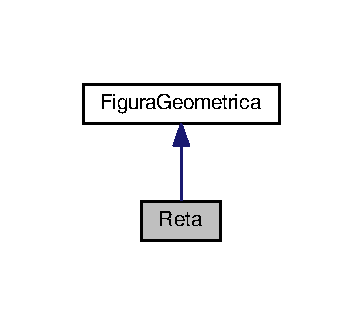
\includegraphics[width=174pt]{class_reta__inherit__graph}
\end{center}
\end{figure}


Collaboration diagram for Reta\+:
\nopagebreak
\begin{figure}[H]
\begin{center}
\leavevmode
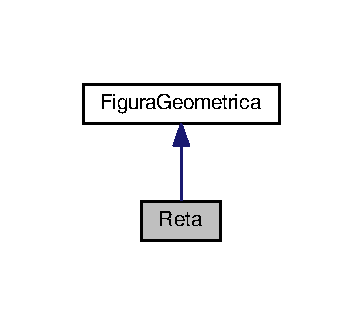
\includegraphics[width=174pt]{class_reta__coll__graph}
\end{center}
\end{figure}
\subsection*{Public Member Functions}
\begin{DoxyCompactItemize}
\item 
\hyperlink{class_reta_a3eea3336e04e4f8acdb9cbb3cafb472a}{Reta} (int \+\_\+xi=0, int \+\_\+yi=0, int \+\_\+xf=0, int \+\_\+yf=0, char \+\_\+brush=\textquotesingle{}$\ast$\textquotesingle{})
\begin{DoxyCompactList}\small\item\em \hyperlink{class_reta}{Reta} é o construtor da classe \hyperlink{class_reta}{Reta}. \end{DoxyCompactList}\item 
void \hyperlink{class_reta_ac2e9805183cd474b62bffd8b032cd780}{draw} (\hyperlink{class_screen}{Screen} \&t)
\begin{DoxyCompactList}\small\item\em draw é uma função que desenha a \hyperlink{class_reta}{Reta} criada numa tela \end{DoxyCompactList}\item 
int \hyperlink{class_reta_a0890517655f27827a827c88850f8984e}{Sinal} (int x)
\begin{DoxyCompactList}\small\item\em Sinal é uma função auxialiar usada no algoritmo de desenhar uma \hyperlink{class_reta}{Reta} digital. \end{DoxyCompactList}\end{DoxyCompactItemize}


\subsection{Detailed Description}
A classe \hyperlink{class_reta}{Reta} cria um objeto do tipo \hyperlink{class_reta}{Reta} que pode ser desenhada numa \hyperlink{class_screen}{Screen}. 

Esta classe extende a classe \hyperlink{class_figura_geometrica}{Figura\+Geometrica} 

\subsection{Constructor \& Destructor Documentation}
\index{Reta@{Reta}!Reta@{Reta}}
\index{Reta@{Reta}!Reta@{Reta}}
\subsubsection[{\texorpdfstring{Reta(int \+\_\+xi=0, int \+\_\+yi=0, int \+\_\+xf=0, int \+\_\+yf=0, char \+\_\+brush=\textquotesingle{}$\ast$\textquotesingle{})}{Reta(int _xi=0, int _yi=0, int _xf=0, int _yf=0, char _brush='*')}}]{\setlength{\rightskip}{0pt plus 5cm}Reta\+::\+Reta (
\begin{DoxyParamCaption}
\item[{int}]{\+\_\+xi = {\ttfamily 0}, }
\item[{int}]{\+\_\+yi = {\ttfamily 0}, }
\item[{int}]{\+\_\+xf = {\ttfamily 0}, }
\item[{int}]{\+\_\+yf = {\ttfamily 0}, }
\item[{char}]{\+\_\+brush = {\ttfamily \textquotesingle{}$\ast$\textquotesingle{}}}
\end{DoxyParamCaption}
)}\hypertarget{class_reta_a3eea3336e04e4f8acdb9cbb3cafb472a}{}\label{class_reta_a3eea3336e04e4f8acdb9cbb3cafb472a}


\hyperlink{class_reta}{Reta} é o construtor da classe \hyperlink{class_reta}{Reta}. 


\begin{DoxyParams}{Parameters}
{\em \+\_\+xi} & é a coordenada x do ponto inicial da \hyperlink{class_reta}{Reta} \\
\hline
{\em \+\_\+yi} & é a coordenada y do ponto inicial da \hyperlink{class_reta}{Reta} \\
\hline
{\em \+\_\+xf} & é a coordenada x do ponto final da \hyperlink{class_reta}{Reta} \\
\hline
{\em \+\_\+yf} & é a coordenada y do ponto final da \hyperlink{class_reta}{Reta} \\
\hline
{\em \+\_\+brush} & é o caractere a ser usado para desenhar a \hyperlink{class_reta}{Reta} \\
\hline
\end{DoxyParams}


\subsection{Member Function Documentation}
\index{Reta@{Reta}!draw@{draw}}
\index{draw@{draw}!Reta@{Reta}}
\subsubsection[{\texorpdfstring{draw(\+Screen \&t)}{draw(Screen &t)}}]{\setlength{\rightskip}{0pt plus 5cm}void Reta\+::draw (
\begin{DoxyParamCaption}
\item[{{\bf Screen} \&}]{t}
\end{DoxyParamCaption}
)\hspace{0.3cm}{\ttfamily [virtual]}}\hypertarget{class_reta_ac2e9805183cd474b62bffd8b032cd780}{}\label{class_reta_ac2e9805183cd474b62bffd8b032cd780}


draw é uma função que desenha a \hyperlink{class_reta}{Reta} criada numa tela 


\begin{DoxyParams}{Parameters}
{\em t} & é a tela na qual se deseja desenhar \\
\hline
\end{DoxyParams}


Implements \hyperlink{class_figura_geometrica_a8ee8dedc060b6059a805ea091aef2c41}{Figura\+Geometrica}.

\index{Reta@{Reta}!Sinal@{Sinal}}
\index{Sinal@{Sinal}!Reta@{Reta}}
\subsubsection[{\texorpdfstring{Sinal(int x)}{Sinal(int x)}}]{\setlength{\rightskip}{0pt plus 5cm}int Reta\+::\+Sinal (
\begin{DoxyParamCaption}
\item[{int}]{x}
\end{DoxyParamCaption}
)}\hypertarget{class_reta_a0890517655f27827a827c88850f8984e}{}\label{class_reta_a0890517655f27827a827c88850f8984e}


Sinal é uma função auxialiar usada no algoritmo de desenhar uma \hyperlink{class_reta}{Reta} digital. 


\begin{DoxyParams}{Parameters}
{\em x} & é um parâmetro usado para o cálculo da reta digital \\
\hline
\end{DoxyParams}
\begin{DoxyReturn}{Returns}
valor inteiro (-\/1, 0 ou 1) que indicará o sinal de uma operação necessária para desenhar a \hyperlink{class_reta}{Reta} 
\end{DoxyReturn}


The documentation for this class was generated from the following files\+:\begin{DoxyCompactItemize}
\item 
\hyperlink{reta_8h}{reta.\+h}\item 
\hyperlink{reta_8cpp}{reta.\+cpp}\end{DoxyCompactItemize}

\hypertarget{class_retangulo}{}\section{Retangulo Class Reference}
\label{class_retangulo}\index{Retangulo@{Retangulo}}


A classe \hyperlink{class_retangulo}{Retangulo} cria um objeto do tipo \hyperlink{class_retangulo}{Retangulo} que pode ser desenhada numa \hyperlink{class_screen}{Screen}.  




{\ttfamily \#include $<$retangulo.\+h$>$}



Inheritance diagram for Retangulo\+:
\nopagebreak
\begin{figure}[H]
\begin{center}
\leavevmode
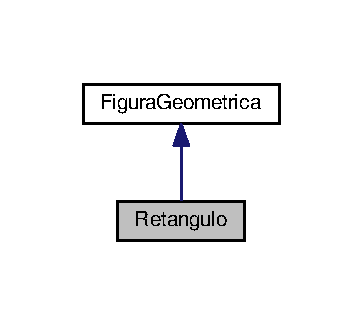
\includegraphics[width=174pt]{class_retangulo__inherit__graph}
\end{center}
\end{figure}


Collaboration diagram for Retangulo\+:
\nopagebreak
\begin{figure}[H]
\begin{center}
\leavevmode
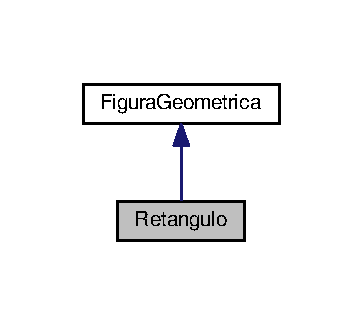
\includegraphics[width=174pt]{class_retangulo__coll__graph}
\end{center}
\end{figure}
\subsection*{Public Member Functions}
\begin{DoxyCompactItemize}
\item 
\hyperlink{class_retangulo_ad1646092a00ba28fcaa8390ce366f3b7}{Retangulo} (int \+\_\+x0=0, int \+\_\+y0=0, int \+\_\+l=0, int \+\_\+a=0, int \+\_\+fillmode=0, char \+\_\+brush=\textquotesingle{}$\ast$\textquotesingle{})
\begin{DoxyCompactList}\small\item\em \hyperlink{class_retangulo}{Retangulo} é o construtor da classe \hyperlink{class_retangulo}{Retangulo}. \end{DoxyCompactList}\item 
void \hyperlink{class_retangulo_ac088dd6d3f4f3d3f80363a868c2e74f1}{draw} (\hyperlink{class_screen}{Screen} \&t)
\begin{DoxyCompactList}\small\item\em draw desenha um \hyperlink{class_retangulo}{Retangulo} numa tela \end{DoxyCompactList}\end{DoxyCompactItemize}


\subsection{Detailed Description}
A classe \hyperlink{class_retangulo}{Retangulo} cria um objeto do tipo \hyperlink{class_retangulo}{Retangulo} que pode ser desenhada numa \hyperlink{class_screen}{Screen}. 

Esta classe extende a classe \hyperlink{class_figura_geometrica}{Figura\+Geometrica} 

\subsection{Constructor \& Destructor Documentation}
\index{Retangulo@{Retangulo}!Retangulo@{Retangulo}}
\index{Retangulo@{Retangulo}!Retangulo@{Retangulo}}
\subsubsection[{\texorpdfstring{Retangulo(int \+\_\+x0=0, int \+\_\+y0=0, int \+\_\+l=0, int \+\_\+a=0, int \+\_\+fillmode=0, char \+\_\+brush=\textquotesingle{}$\ast$\textquotesingle{})}{Retangulo(int _x0=0, int _y0=0, int _l=0, int _a=0, int _fillmode=0, char _brush='*')}}]{\setlength{\rightskip}{0pt plus 5cm}Retangulo\+::\+Retangulo (
\begin{DoxyParamCaption}
\item[{int}]{\+\_\+x0 = {\ttfamily 0}, }
\item[{int}]{\+\_\+y0 = {\ttfamily 0}, }
\item[{int}]{\+\_\+l = {\ttfamily 0}, }
\item[{int}]{\+\_\+a = {\ttfamily 0}, }
\item[{int}]{\+\_\+fillmode = {\ttfamily 0}, }
\item[{char}]{\+\_\+brush = {\ttfamily \textquotesingle{}$\ast$\textquotesingle{}}}
\end{DoxyParamCaption}
)}\hypertarget{class_retangulo_ad1646092a00ba28fcaa8390ce366f3b7}{}\label{class_retangulo_ad1646092a00ba28fcaa8390ce366f3b7}


\hyperlink{class_retangulo}{Retangulo} é o construtor da classe \hyperlink{class_retangulo}{Retangulo}. 


\begin{DoxyParams}{Parameters}
{\em \+\_\+x0} & é o valor da coordenada x do ponto superior esquerdo do \hyperlink{class_retangulo}{Retangulo} \\
\hline
{\em \+\_\+y0} & é o valor da coordenada y do ponto superior esquerdo do \hyperlink{class_retangulo}{Retangulo} \\
\hline
{\em \+\_\+l} & é o valor da largura do \hyperlink{class_retangulo}{Retangulo} \\
\hline
{\em \+\_\+a} & é o valor da altura do \hyperlink{class_retangulo}{Retangulo} \\
\hline
{\em \+\_\+fillmode} & indica se o \hyperlink{class_retangulo}{Retangulo} deve ser preenchido ou não \\
\hline
{\em \+\_\+brush} & indica o caractere a ser usado para desenhar o \hyperlink{class_retangulo}{Retangulo} uma tela \\
\hline
\end{DoxyParams}


\subsection{Member Function Documentation}
\index{Retangulo@{Retangulo}!draw@{draw}}
\index{draw@{draw}!Retangulo@{Retangulo}}
\subsubsection[{\texorpdfstring{draw(\+Screen \&t)}{draw(Screen &t)}}]{\setlength{\rightskip}{0pt plus 5cm}void Retangulo\+::draw (
\begin{DoxyParamCaption}
\item[{{\bf Screen} \&}]{t}
\end{DoxyParamCaption}
)\hspace{0.3cm}{\ttfamily [virtual]}}\hypertarget{class_retangulo_ac088dd6d3f4f3d3f80363a868c2e74f1}{}\label{class_retangulo_ac088dd6d3f4f3d3f80363a868c2e74f1}


draw desenha um \hyperlink{class_retangulo}{Retangulo} numa tela 


\begin{DoxyParams}{Parameters}
{\em t} & é a tela na qual se deseja desenhar \\
\hline
\end{DoxyParams}


Implements \hyperlink{class_figura_geometrica_a8ee8dedc060b6059a805ea091aef2c41}{Figura\+Geometrica}.



The documentation for this class was generated from the following files\+:\begin{DoxyCompactItemize}
\item 
\hyperlink{retangulo_8h}{retangulo.\+h}\item 
\hyperlink{retangulo_8cpp}{retangulo.\+cpp}\end{DoxyCompactItemize}

\hypertarget{class_screen}{}\section{Screen Class Reference}
\label{class_screen}\index{Screen@{Screen}}


A classe \hyperlink{class_screen}{Screen} exibe imagens numa tela.  




{\ttfamily \#include $<$screen.\+h$>$}

\subsection*{Public Member Functions}
\begin{DoxyCompactItemize}
\item 
\hyperlink{class_screen_a95aff497d133f685fbbb959d78dc0899}{Screen} (int \+\_\+nlin=10, int \+\_\+ncol=10)
\begin{DoxyCompactList}\small\item\em \hyperlink{class_screen}{Screen} é o construtor da classe \hyperlink{class_screen}{Screen}. \end{DoxyCompactList}\item 
void \hyperlink{class_screen_ae6bea81c57a22d226507c3c26fa95ee0}{set\+Pixel} (int x, int y)
\begin{DoxyCompactList}\small\item\em set\+Pixel altera o conteúdo de um pixel da tela \end{DoxyCompactList}\item 
void \hyperlink{class_screen_a35e74266b2a04e37b354ceff7a5f1031}{clear} ()
\begin{DoxyCompactList}\small\item\em clear limpa a tela deixando-\/a em branco \end{DoxyCompactList}\item 
void \hyperlink{class_screen_a59f2c3f9e889b425940749e8f646db72}{set\+Screen} (int nl, int nc)
\begin{DoxyCompactList}\small\item\em set\+Screen altera as dismensões da tela \end{DoxyCompactList}\item 
void \hyperlink{class_screen_aad52e3e6f35fe32f185cd70550a0a305}{set\+Brush} (char \+\_\+brush= \textquotesingle{}$\ast$\textquotesingle{})
\begin{DoxyCompactList}\small\item\em set\+Brush altera o pincel usado para desenhar na tela \end{DoxyCompactList}\end{DoxyCompactItemize}
\subsection*{Friends}
\begin{DoxyCompactItemize}
\item 
ostream \& \hyperlink{class_screen_aab6a2880746bfe1b7964817cc8f0989e}{operator$<$$<$} (ostream \&os, \hyperlink{class_screen}{Screen} \&t)
\begin{DoxyCompactList}\small\item\em operator $<$$<$ é a sobrecarga do operador $<$$<$ \end{DoxyCompactList}\end{DoxyCompactItemize}


\subsection{Detailed Description}
A classe \hyperlink{class_screen}{Screen} exibe imagens numa tela. 

\subsection{Constructor \& Destructor Documentation}
\index{Screen@{Screen}!Screen@{Screen}}
\index{Screen@{Screen}!Screen@{Screen}}
\subsubsection[{\texorpdfstring{Screen(int \+\_\+nlin=10, int \+\_\+ncol=10)}{Screen(int _nlin=10, int _ncol=10)}}]{\setlength{\rightskip}{0pt plus 5cm}Screen\+::\+Screen (
\begin{DoxyParamCaption}
\item[{int}]{\+\_\+nlin = {\ttfamily 10}, }
\item[{int}]{\+\_\+ncol = {\ttfamily 10}}
\end{DoxyParamCaption}
)}\hypertarget{class_screen_a95aff497d133f685fbbb959d78dc0899}{}\label{class_screen_a95aff497d133f685fbbb959d78dc0899}


\hyperlink{class_screen}{Screen} é o construtor da classe \hyperlink{class_screen}{Screen}. 


\begin{DoxyParams}{Parameters}
{\em \+\_\+nlin} & é o número de linhas da tela, ou seja, a altura (dimensão Y) \\
\hline
{\em \+\_\+ncol} & é o número de colunas da tela, ou seja, a largura (dimensão X) \\
\hline
\end{DoxyParams}


\subsection{Member Function Documentation}
\index{Screen@{Screen}!clear@{clear}}
\index{clear@{clear}!Screen@{Screen}}
\subsubsection[{\texorpdfstring{clear()}{clear()}}]{\setlength{\rightskip}{0pt plus 5cm}void Screen\+::clear (
\begin{DoxyParamCaption}
{}
\end{DoxyParamCaption}
)}\hypertarget{class_screen_a35e74266b2a04e37b354ceff7a5f1031}{}\label{class_screen_a35e74266b2a04e37b354ceff7a5f1031}


clear limpa a tela deixando-\/a em branco 

\index{Screen@{Screen}!set\+Brush@{set\+Brush}}
\index{set\+Brush@{set\+Brush}!Screen@{Screen}}
\subsubsection[{\texorpdfstring{set\+Brush(char \+\_\+brush= \textquotesingle{}$\ast$\textquotesingle{})}{setBrush(char _brush= '*')}}]{\setlength{\rightskip}{0pt plus 5cm}void Screen\+::set\+Brush (
\begin{DoxyParamCaption}
\item[{char}]{\+\_\+brush = {\ttfamily \textquotesingle{}$\ast$\textquotesingle{}}}
\end{DoxyParamCaption}
)}\hypertarget{class_screen_aad52e3e6f35fe32f185cd70550a0a305}{}\label{class_screen_aad52e3e6f35fe32f185cd70550a0a305}


set\+Brush altera o pincel usado para desenhar na tela 


\begin{DoxyParams}{Parameters}
{\em \+\_\+brush} & é o parâmetro que recebe o caracetere a ser usado para o pincel \\
\hline
\end{DoxyParams}
\index{Screen@{Screen}!set\+Pixel@{set\+Pixel}}
\index{set\+Pixel@{set\+Pixel}!Screen@{Screen}}
\subsubsection[{\texorpdfstring{set\+Pixel(int x, int y)}{setPixel(int x, int y)}}]{\setlength{\rightskip}{0pt plus 5cm}void Screen\+::set\+Pixel (
\begin{DoxyParamCaption}
\item[{int}]{x, }
\item[{int}]{y}
\end{DoxyParamCaption}
)}\hypertarget{class_screen_ae6bea81c57a22d226507c3c26fa95ee0}{}\label{class_screen_ae6bea81c57a22d226507c3c26fa95ee0}


set\+Pixel altera o conteúdo de um pixel da tela 


\begin{DoxyParams}{Parameters}
{\em x} & é a coordenada x do pixel a ser alterado \\
\hline
{\em y} & é a coordenada y do pixel a ser alterado \\
\hline
\end{DoxyParams}
\index{Screen@{Screen}!set\+Screen@{set\+Screen}}
\index{set\+Screen@{set\+Screen}!Screen@{Screen}}
\subsubsection[{\texorpdfstring{set\+Screen(int nl, int nc)}{setScreen(int nl, int nc)}}]{\setlength{\rightskip}{0pt plus 5cm}void Screen\+::set\+Screen (
\begin{DoxyParamCaption}
\item[{int}]{nl, }
\item[{int}]{nc}
\end{DoxyParamCaption}
)}\hypertarget{class_screen_a59f2c3f9e889b425940749e8f646db72}{}\label{class_screen_a59f2c3f9e889b425940749e8f646db72}


set\+Screen altera as dismensões da tela 


\begin{DoxyParams}{Parameters}
{\em nl} & é o número de linhas a ser setado \\
\hline
{\em nc} & é o número de colunas a ser setado \\
\hline
\end{DoxyParams}


\subsection{Friends And Related Function Documentation}
\index{Screen@{Screen}!operator$<$$<$@{operator$<$$<$}}
\index{operator$<$$<$@{operator$<$$<$}!Screen@{Screen}}
\subsubsection[{\texorpdfstring{operator$<$$<$}{operator<<}}]{\setlength{\rightskip}{0pt plus 5cm}ostream\& operator$<$$<$ (
\begin{DoxyParamCaption}
\item[{ostream \&}]{os, }
\item[{{\bf Screen} \&}]{t}
\end{DoxyParamCaption}
)\hspace{0.3cm}{\ttfamily [friend]}}\hypertarget{class_screen_aab6a2880746bfe1b7964817cc8f0989e}{}\label{class_screen_aab6a2880746bfe1b7964817cc8f0989e}


operator $<$$<$ é a sobrecarga do operador $<$$<$ 


\begin{DoxyParams}{Parameters}
{\em os} & é um parâmetro de fluxos de saída \\
\hline
{\em t} & é a tela na qual deve ser desenhada \\
\hline
\end{DoxyParams}
\begin{DoxyReturn}{Returns}

\end{DoxyReturn}


The documentation for this class was generated from the following files\+:\begin{DoxyCompactItemize}
\item 
\hyperlink{screen_8h}{screen.\+h}\item 
\hyperlink{screen_8cpp}{screen.\+cpp}\end{DoxyCompactItemize}

\chapter{File Documentation}
\hypertarget{circulo_8cpp}{}\section{circulo.\+cpp File Reference}
\label{circulo_8cpp}\index{circulo.\+cpp@{circulo.\+cpp}}
{\ttfamily \#include \char`\"{}circulo.\+h\char`\"{}}\\*
{\ttfamily \#include \char`\"{}screen.\+h\char`\"{}}\\*
{\ttfamily \#include $<$iostream$>$}\\*
Include dependency graph for circulo.\+cpp\+:
\nopagebreak
\begin{figure}[H]
\begin{center}
\leavevmode
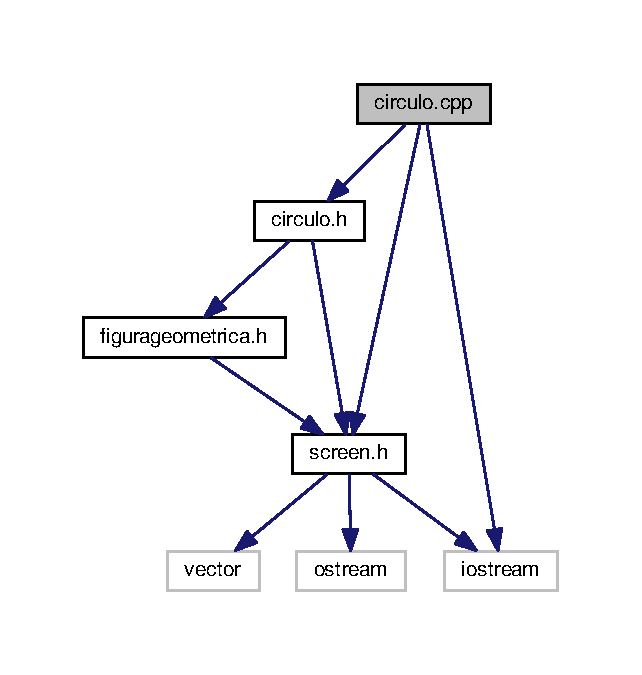
\includegraphics[width=308pt]{circulo_8cpp__incl}
\end{center}
\end{figure}

\hypertarget{circulo_8h}{}\section{circulo.\+h File Reference}
\label{circulo_8h}\index{circulo.\+h@{circulo.\+h}}
{\ttfamily \#include \char`\"{}figurageometrica.\+h\char`\"{}}\\*
{\ttfamily \#include \char`\"{}screen.\+h\char`\"{}}\\*
Include dependency graph for circulo.\+h\+:
\nopagebreak
\begin{figure}[H]
\begin{center}
\leavevmode
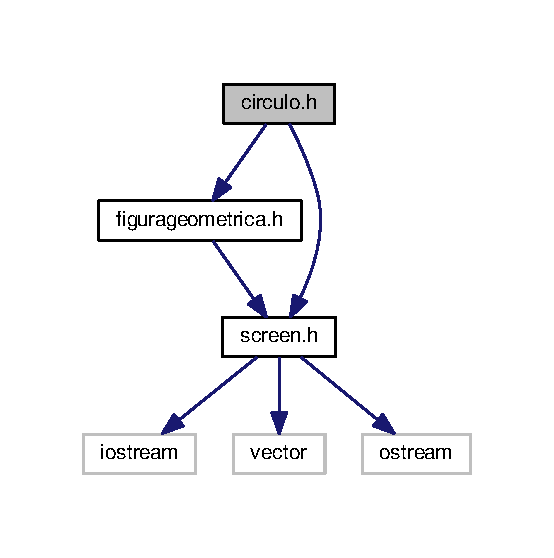
\includegraphics[width=266pt]{circulo_8h__incl}
\end{center}
\end{figure}
This graph shows which files directly or indirectly include this file\+:
\nopagebreak
\begin{figure}[H]
\begin{center}
\leavevmode
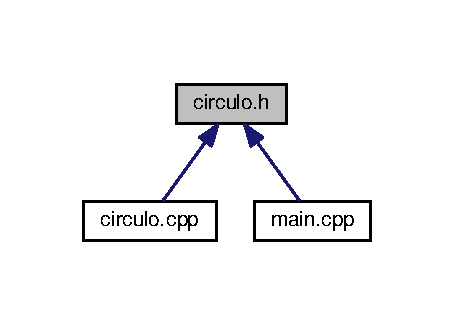
\includegraphics[width=218pt]{circulo_8h__dep__incl}
\end{center}
\end{figure}
\subsection*{Classes}
\begin{DoxyCompactItemize}
\item 
class \hyperlink{class_circulo}{Circulo}
\begin{DoxyCompactList}\small\item\em A classe \hyperlink{class_circulo}{Circulo} cria um objeto do tipo \hyperlink{class_circulo}{Circulo} que pode ser desenhada numa \hyperlink{class_screen}{Screen}. \end{DoxyCompactList}\end{DoxyCompactItemize}

\hypertarget{figurageometrica_8cpp}{}\section{figurageometrica.\+cpp File Reference}
\label{figurageometrica_8cpp}\index{figurageometrica.\+cpp@{figurageometrica.\+cpp}}
{\ttfamily \#include \char`\"{}figurageometrica.\+h\char`\"{}}\\*
Include dependency graph for figurageometrica.\+cpp\+:
\nopagebreak
\begin{figure}[H]
\begin{center}
\leavevmode
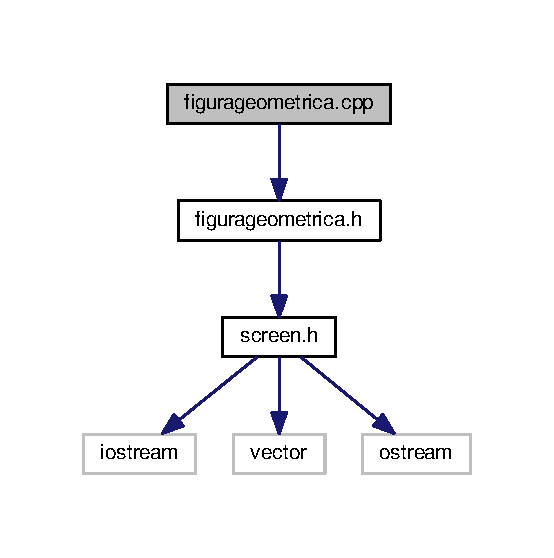
\includegraphics[width=266pt]{figurageometrica_8cpp__incl}
\end{center}
\end{figure}

\hypertarget{figurageometrica_8h}{}\section{figurageometrica.\+h File Reference}
\label{figurageometrica_8h}\index{figurageometrica.\+h@{figurageometrica.\+h}}
{\ttfamily \#include \char`\"{}screen.\+h\char`\"{}}\\*
Include dependency graph for figurageometrica.\+h\+:
\nopagebreak
\begin{figure}[H]
\begin{center}
\leavevmode
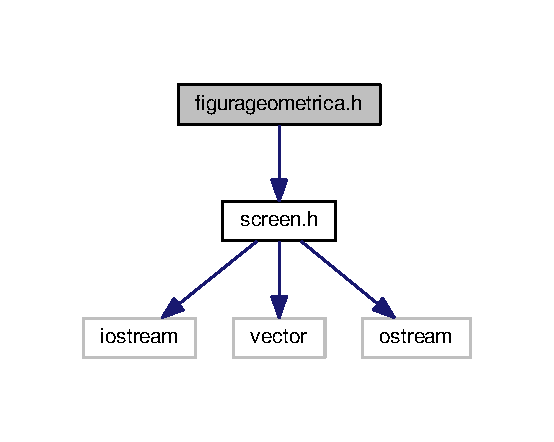
\includegraphics[width=266pt]{figurageometrica_8h__incl}
\end{center}
\end{figure}
This graph shows which files directly or indirectly include this file\+:
\nopagebreak
\begin{figure}[H]
\begin{center}
\leavevmode
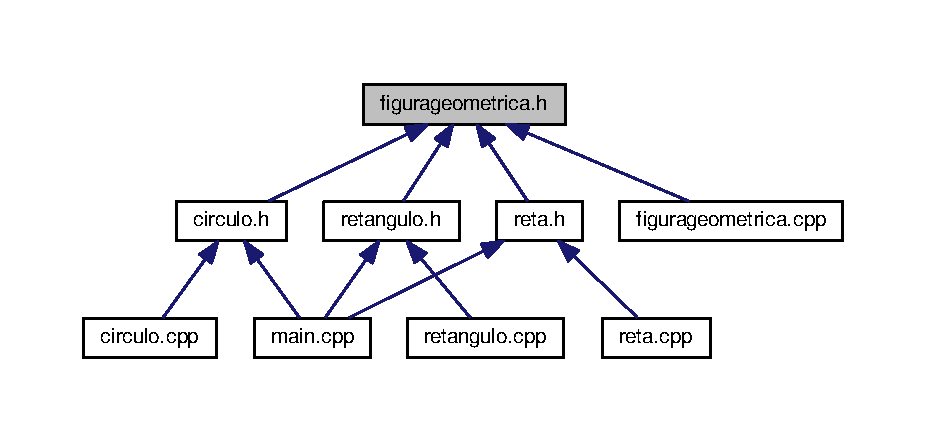
\includegraphics[width=350pt]{figurageometrica_8h__dep__incl}
\end{center}
\end{figure}
\subsection*{Classes}
\begin{DoxyCompactItemize}
\item 
class \hyperlink{class_figura_geometrica}{Figura\+Geometrica}
\begin{DoxyCompactList}\small\item\em A classe \hyperlink{class_figura_geometrica}{Figura\+Geometrica} é uma classe abstrata que desenha Figuras Geometricas. \end{DoxyCompactList}\end{DoxyCompactItemize}

\hypertarget{main_8cpp}{}\section{Qt\+Tcp\+Server/main.cpp File Reference}
\label{main_8cpp}\index{Qt\+Tcp\+Server/main.\+cpp@{Qt\+Tcp\+Server/main.\+cpp}}
{\ttfamily \#include \char`\"{}mainwindow.\+h\char`\"{}}\\*
{\ttfamily \#include $<$Q\+Application$>$}\\*
Include dependency graph for main.\+cpp\+:
\nopagebreak
\begin{figure}[H]
\begin{center}
\leavevmode
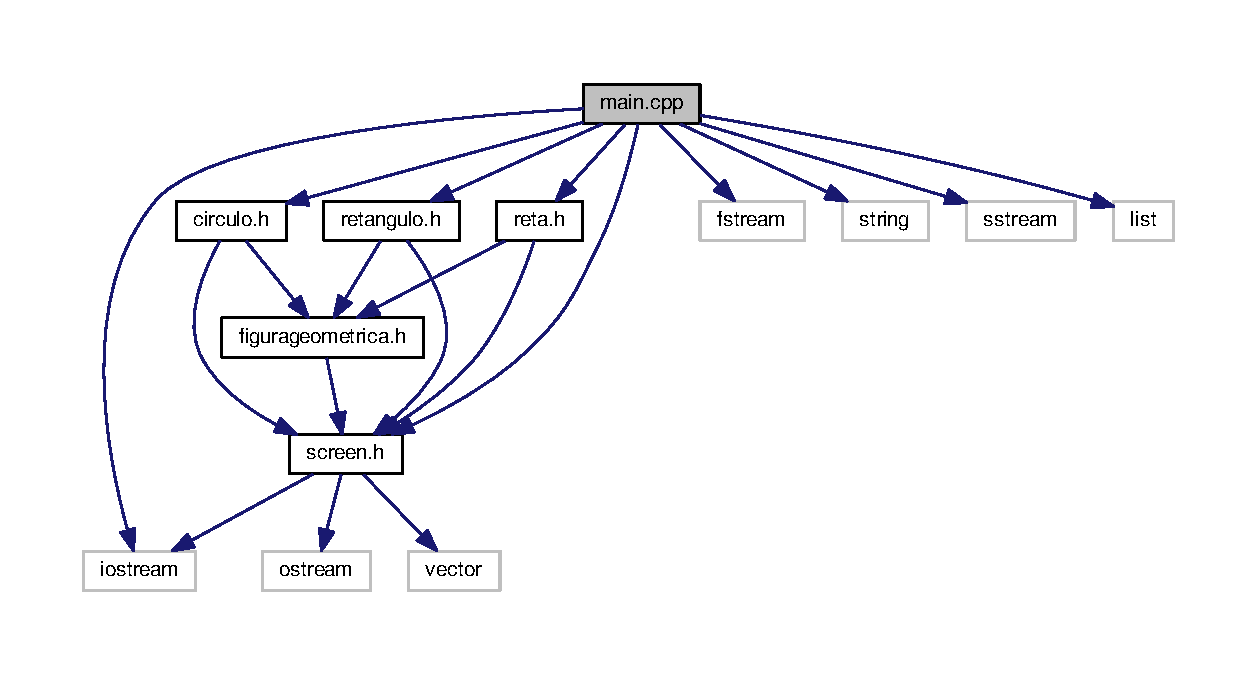
\includegraphics[width=350pt]{main_8cpp__incl}
\end{center}
\end{figure}
\subsection*{Functions}
\begin{DoxyCompactItemize}
\item 
int \hyperlink{main_8cpp_a0ddf1224851353fc92bfbff6f499fa97}{main} (int argc, char $\ast$argv\mbox{[}$\,$\mbox{]})
\end{DoxyCompactItemize}


\subsection{Function Documentation}
\index{main.\+cpp@{main.\+cpp}!main@{main}}
\index{main@{main}!main.\+cpp@{main.\+cpp}}
\subsubsection[{\texorpdfstring{main(int argc, char $\ast$argv[])}{main(int argc, char *argv[])}}]{\setlength{\rightskip}{0pt plus 5cm}int main (
\begin{DoxyParamCaption}
\item[{int}]{argc, }
\item[{char $\ast$}]{argv\mbox{[}$\,$\mbox{]}}
\end{DoxyParamCaption}
)}\hypertarget{main_8cpp_a0ddf1224851353fc92bfbff6f499fa97}{}\label{main_8cpp_a0ddf1224851353fc92bfbff6f499fa97}

\hypertarget{_r_e_a_d_m_e_8md}{}\section{R\+E\+A\+D\+M\+E.\+md File Reference}
\label{_r_e_a_d_m_e_8md}\index{R\+E\+A\+D\+M\+E.\+md@{R\+E\+A\+D\+M\+E.\+md}}

\hypertarget{reta_8cpp}{}\section{reta.\+cpp File Reference}
\label{reta_8cpp}\index{reta.\+cpp@{reta.\+cpp}}
{\ttfamily \#include \char`\"{}reta.\+h\char`\"{}}\\*
{\ttfamily \#include \char`\"{}screen.\+h\char`\"{}}\\*
{\ttfamily \#include $<$iostream$>$}\\*
{\ttfamily \#include $<$stdlib.\+h$>$}\\*
Include dependency graph for reta.\+cpp\+:
\nopagebreak
\begin{figure}[H]
\begin{center}
\leavevmode
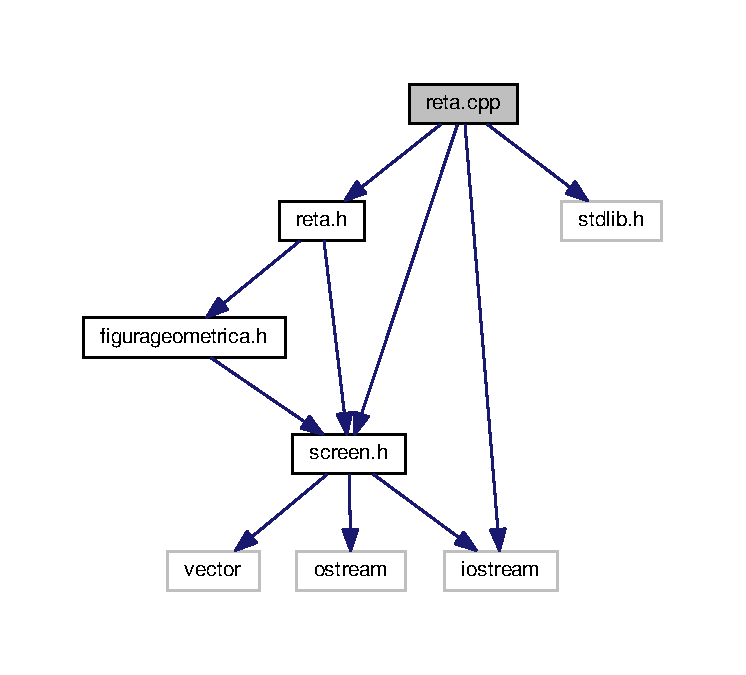
\includegraphics[width=350pt]{reta_8cpp__incl}
\end{center}
\end{figure}

\hypertarget{reta_8h}{}\section{reta.\+h File Reference}
\label{reta_8h}\index{reta.\+h@{reta.\+h}}
{\ttfamily \#include \char`\"{}figurageometrica.\+h\char`\"{}}\\*
{\ttfamily \#include \char`\"{}screen.\+h\char`\"{}}\\*
Include dependency graph for reta.\+h\+:
\nopagebreak
\begin{figure}[H]
\begin{center}
\leavevmode
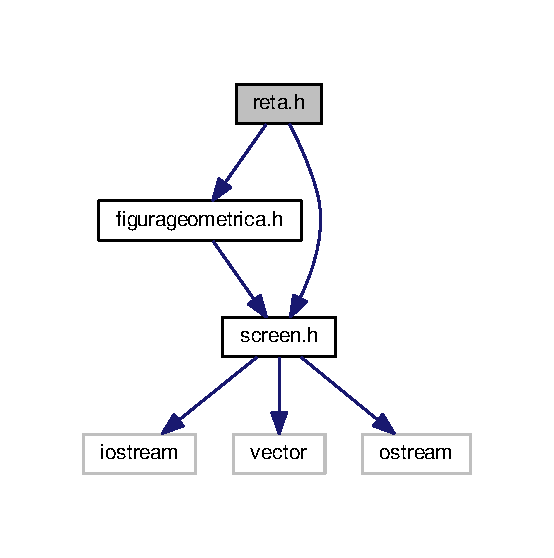
\includegraphics[width=266pt]{reta_8h__incl}
\end{center}
\end{figure}
This graph shows which files directly or indirectly include this file\+:
\nopagebreak
\begin{figure}[H]
\begin{center}
\leavevmode
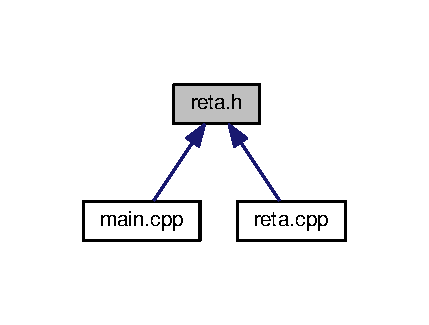
\includegraphics[width=206pt]{reta_8h__dep__incl}
\end{center}
\end{figure}
\subsection*{Classes}
\begin{DoxyCompactItemize}
\item 
class \hyperlink{class_reta}{Reta}
\begin{DoxyCompactList}\small\item\em A classe \hyperlink{class_reta}{Reta} cria um objeto do tipo \hyperlink{class_reta}{Reta} que pode ser desenhada numa \hyperlink{class_screen}{Screen}. \end{DoxyCompactList}\end{DoxyCompactItemize}

\hypertarget{retangulo_8cpp}{}\section{retangulo.\+cpp File Reference}
\label{retangulo_8cpp}\index{retangulo.\+cpp@{retangulo.\+cpp}}
{\ttfamily \#include \char`\"{}retangulo.\+h\char`\"{}}\\*
Include dependency graph for retangulo.\+cpp\+:
\nopagebreak
\begin{figure}[H]
\begin{center}
\leavevmode
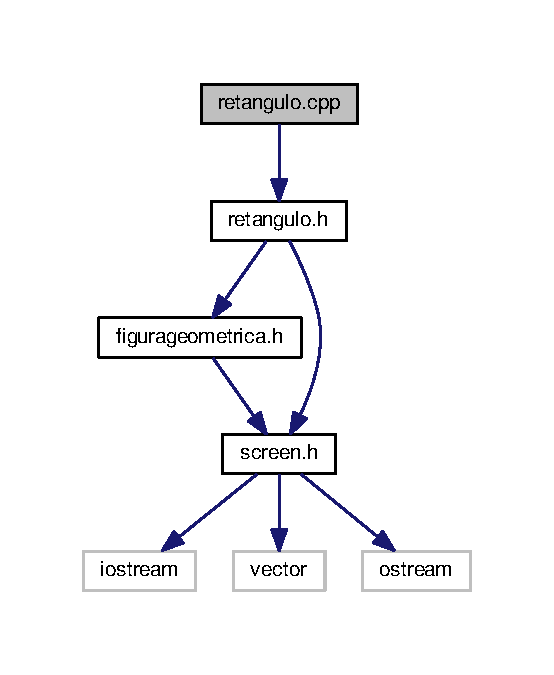
\includegraphics[width=266pt]{retangulo_8cpp__incl}
\end{center}
\end{figure}

\hypertarget{retangulo_8h}{}\section{retangulo.\+h File Reference}
\label{retangulo_8h}\index{retangulo.\+h@{retangulo.\+h}}
{\ttfamily \#include \char`\"{}poligono.\+h\char`\"{}}\\*
Include dependency graph for retangulo.\+h\+:\nopagebreak
\begin{figure}[H]
\begin{center}
\leavevmode
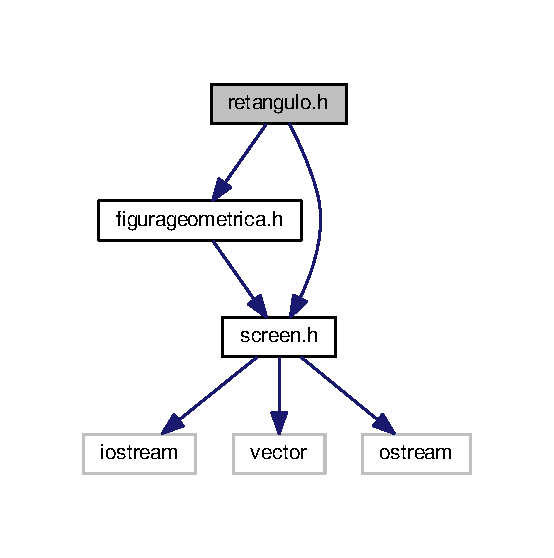
\includegraphics[width=202pt]{retangulo_8h__incl}
\end{center}
\end{figure}
This graph shows which files directly or indirectly include this file\+:\nopagebreak
\begin{figure}[H]
\begin{center}
\leavevmode
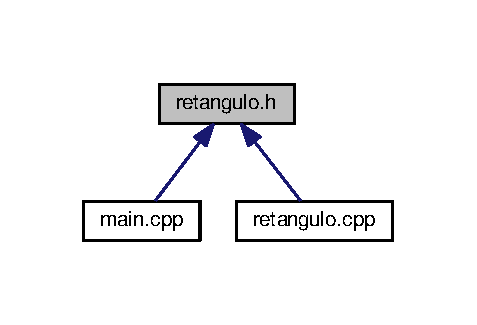
\includegraphics[width=229pt]{retangulo_8h__dep__incl}
\end{center}
\end{figure}
\subsection*{Classes}
\begin{DoxyCompactItemize}
\item 
class \hyperlink{class_retangulo}{Retangulo}
\begin{DoxyCompactList}\small\item\em A classe \hyperlink{class_retangulo}{Retangulo} é uma subclasse da classe \hyperlink{class_poligono}{Poligono} que representa retângulos. \end{DoxyCompactList}\end{DoxyCompactItemize}

\hypertarget{screen_8cpp}{}\section{screen.\+cpp File Reference}
\label{screen_8cpp}\index{screen.\+cpp@{screen.\+cpp}}
{\ttfamily \#include \char`\"{}screen.\+h\char`\"{}}\\*
{\ttfamily \#include $<$iostream$>$}\\*
Include dependency graph for screen.\+cpp\+:
\nopagebreak
\begin{figure}[H]
\begin{center}
\leavevmode
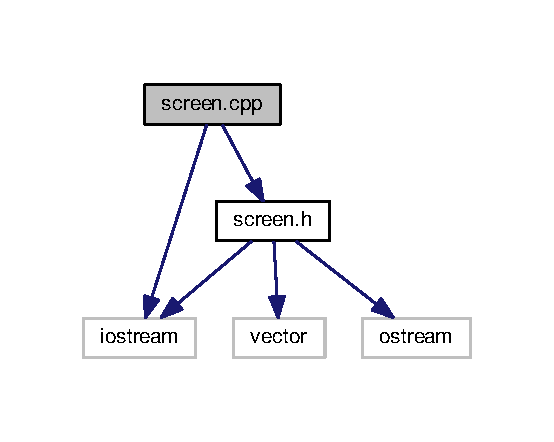
\includegraphics[width=266pt]{screen_8cpp__incl}
\end{center}
\end{figure}
\subsection*{Functions}
\begin{DoxyCompactItemize}
\item 
ostream \& \hyperlink{screen_8cpp_aab6a2880746bfe1b7964817cc8f0989e}{operator$<$$<$} (ostream \&os, \hyperlink{class_screen}{Screen} \&t)
\end{DoxyCompactItemize}


\subsection{Function Documentation}
\index{screen.\+cpp@{screen.\+cpp}!operator$<$$<$@{operator$<$$<$}}
\index{operator$<$$<$@{operator$<$$<$}!screen.\+cpp@{screen.\+cpp}}
\subsubsection[{\texorpdfstring{operator$<$$<$(ostream \&os, Screen \&t)}{operator<<(ostream &os, Screen &t)}}]{\setlength{\rightskip}{0pt plus 5cm}ostream\& operator$<$$<$ (
\begin{DoxyParamCaption}
\item[{ostream \&}]{os, }
\item[{{\bf Screen} \&}]{t}
\end{DoxyParamCaption}
)}\hypertarget{screen_8cpp_aab6a2880746bfe1b7964817cc8f0989e}{}\label{screen_8cpp_aab6a2880746bfe1b7964817cc8f0989e}

\begin{DoxyParams}{Parameters}
{\em os} & é um parâmetro de fluxos de saída \\
\hline
{\em t} & é a tela na qual deve ser desenhada \\
\hline
\end{DoxyParams}
\begin{DoxyReturn}{Returns}

\end{DoxyReturn}

\hypertarget{screen_8h}{}\section{screen.\+h File Reference}
\label{screen_8h}\index{screen.\+h@{screen.\+h}}
{\ttfamily \#include $<$iostream$>$}\\*
{\ttfamily \#include $<$vector$>$}\\*
{\ttfamily \#include $<$ostream$>$}\\*
Include dependency graph for screen.\+h\+:
\nopagebreak
\begin{figure}[H]
\begin{center}
\leavevmode
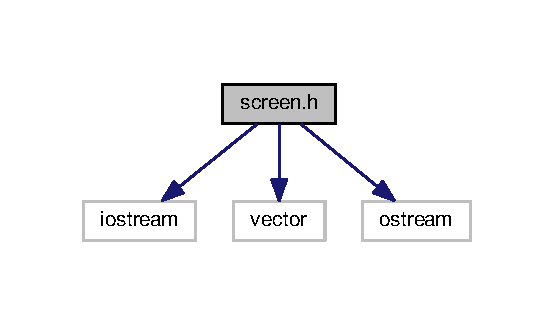
\includegraphics[width=266pt]{screen_8h__incl}
\end{center}
\end{figure}
This graph shows which files directly or indirectly include this file\+:
\nopagebreak
\begin{figure}[H]
\begin{center}
\leavevmode
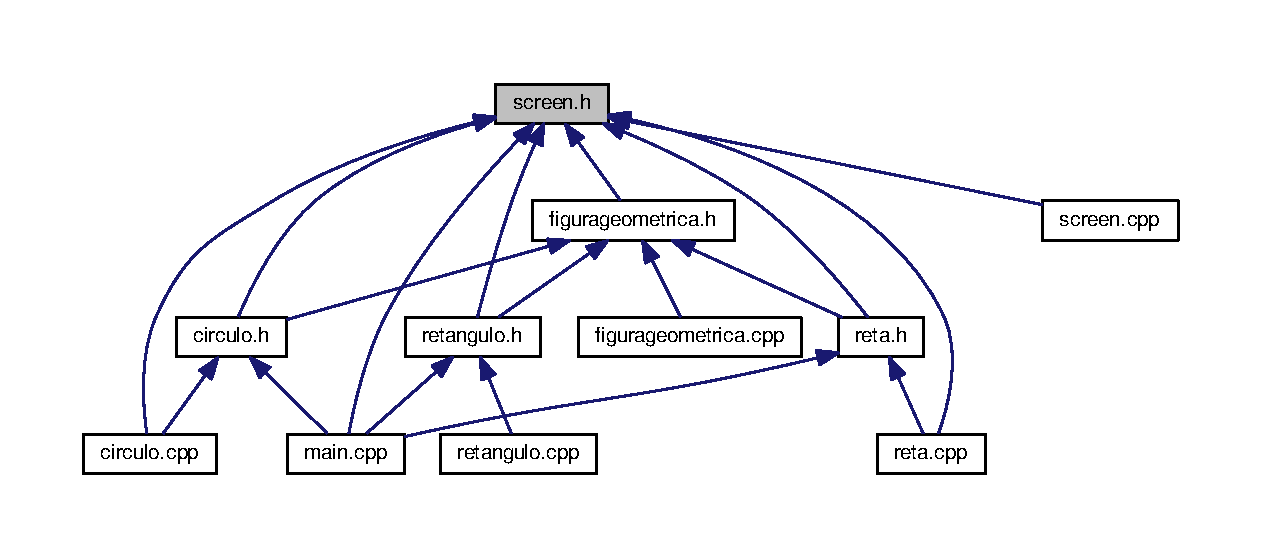
\includegraphics[width=350pt]{screen_8h__dep__incl}
\end{center}
\end{figure}
\subsection*{Classes}
\begin{DoxyCompactItemize}
\item 
class \hyperlink{class_screen}{Screen}
\begin{DoxyCompactList}\small\item\em A classe \hyperlink{class_screen}{Screen} exibe imagens numa tela. \end{DoxyCompactList}\end{DoxyCompactItemize}

%--- End generated contents ---

% Index
\backmatter
\newpage
\phantomsection
\clearemptydoublepage
\addcontentsline{toc}{chapter}{Index}
\printindex

\end{document}
